\appendix
\chapter*{Appendix}
\phantomsection
\addcontentsline{toc}{chapter}{Appendix}
\renewcommand{\thesection}{\Alph{section}}

\section{Lists}

\subsection{List of implemented projects}

\begin{itemize}
\item diplomatiq-frontend: \emph{https://github.com/Diplomatiq/diplomatiq-frontend}
\item diplomatiq-backend: \emph{https://github.com/Diplomatiq/diplomatiq-backend}
\item website: \emph{https://github.com/Diplomatiq/website}
\item crypto-random: \emph{https://github.com/Diplomatiq/crypto-random}
\item resily: \emph{https://github.com/Diplomatiq/resily}
\item convertibles: \emph{https://github.com/Diplomatiq/convertibles}
\item eslint-config-tslib: \emph{https://github.com/Diplomatiq/eslint-config-tslib}
\item eslint-config-angular: \emph{https://github.com/Diplomatiq/eslint-config-angular}
\item project-config: \emph{https://github.com/Diplomatiq/project-config}
\end{itemize}

\section{Tables}

\subsection{Email addresses configured for diplomatiq.org}

\begin{table}[!htb]
    \footnotesize
    \begin{tabular}{l|l|l}
        \toprule
        \textbf{Email address}      & \textbf{Usage}            & \textbf{Notes} \\
        \midrule
        billing@diplomatiq.org     & sending \& receiving      & for billing-related notifications \\
        ceo@diplomatiq.org         & sending \& receiving      & for communicating as the CEO \\
        conduct@diplomatiq.org     & receiving                 & for Code of Conduct violations \\
        github@diplomatiq.org      & sending \& receiving      & for the GitHub service \\
        info@diplomatiq.org        & receiving                 & for personal inquiries \\
        npm@diplomatiq.org         & sending \& receiving      & for Microsoft services \\
        npm@diplomatiq.org         & sending \& receiving      & for the NPM service \\
        security@diplomatiq.org    & receiving                 & for security inquiries \\
        soma.lucz@diplomatiq.org   & sending \& receiving      & for communicating as myself \\
        team@diplomatiq.org        & sending                   & for sending transactional email \\
        \bottomrule
    \end{tabular}
\end{table}

\newpage

\section{Figures}

\subsection{Server calls for elevating a session to password assurance level}

\begin{figure}[!htb]
    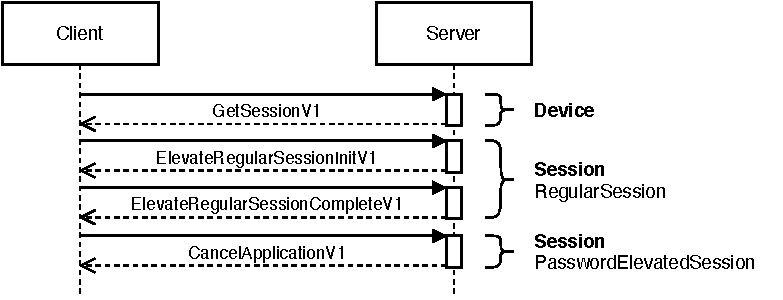
\includegraphics[width=\textwidth]{figures/elevate-to-password-session.pdf}
\end{figure}

\subsection{Server calls for elevating a session to multi-factor assurance level}

\begin{figure}[!htb]
    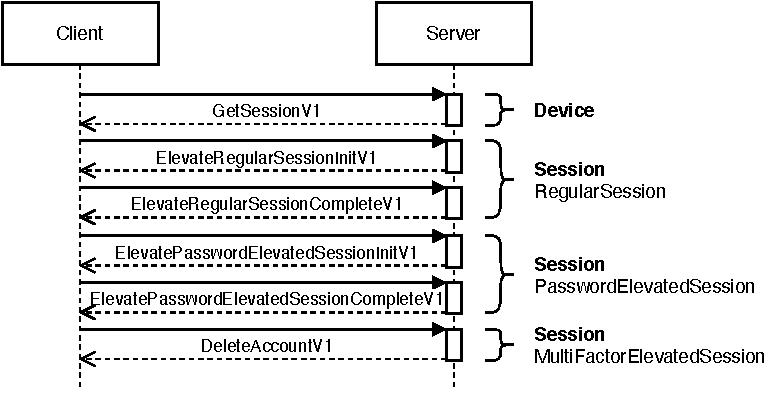
\includegraphics[width=\textwidth]{figures/elevate-to-mfa-session.pdf}
\end{figure}

\newpage

\subsection{Operation of the base headers checker filter}

\begin{figure}[!htb]
    \centering
    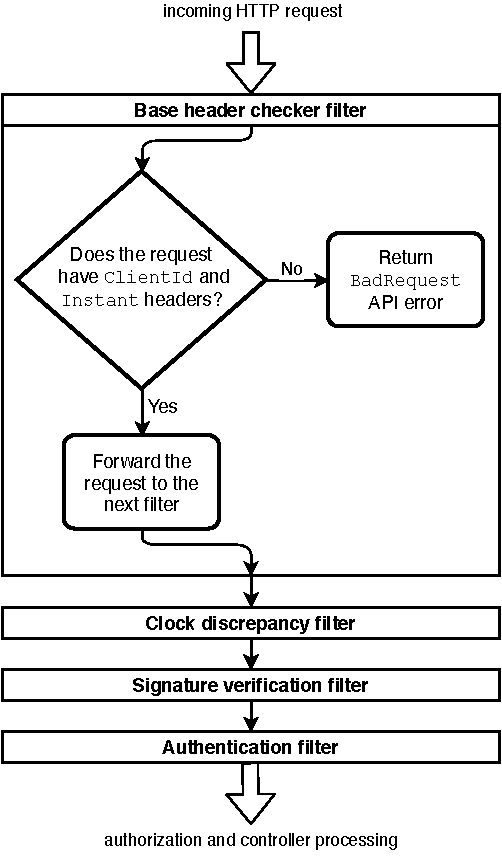
\includegraphics[height=\textheight-1cm]{figures/base-headers-checker-filter.pdf}
\end{figure}

\newpage

\subsection{Operation of the clock discrepancy filter}

\begin{figure}[!htb]
    \centering
    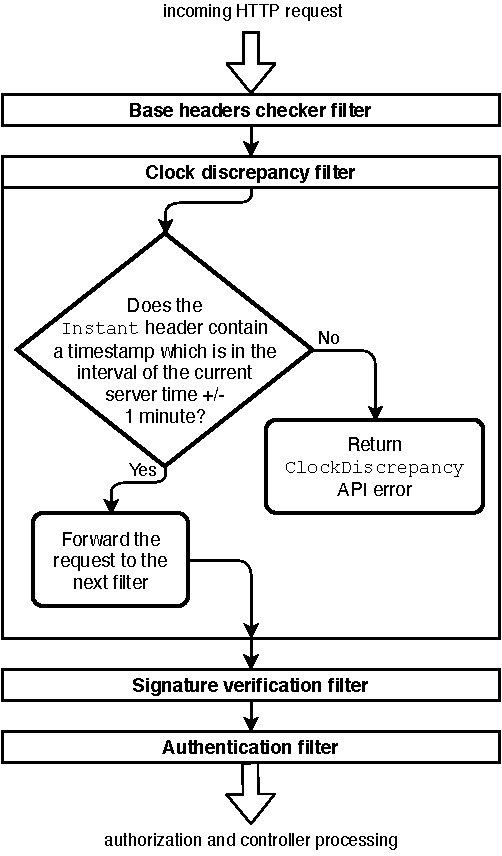
\includegraphics[height=\textheight-1cm]{figures/clock-discrepancy-filter.pdf}
\end{figure}

\newpage

\subsection{Operation of the signature verification filter}

\begin{figure}[!htb]
    \centering
    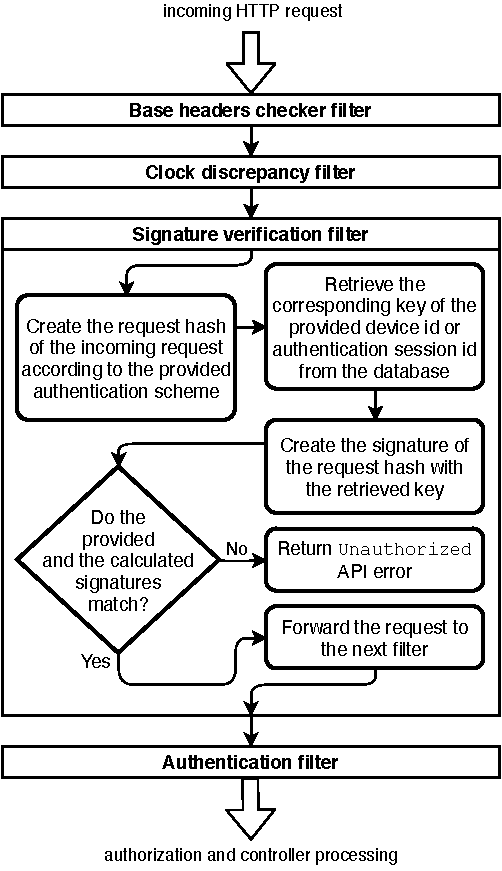
\includegraphics[height=\textheight-1cm]{figures/signature-verification-filter.pdf}
\end{figure}

\newpage

\subsection{Operation of the authentication filter}

\begin{figure}[!htb]
    \centering
    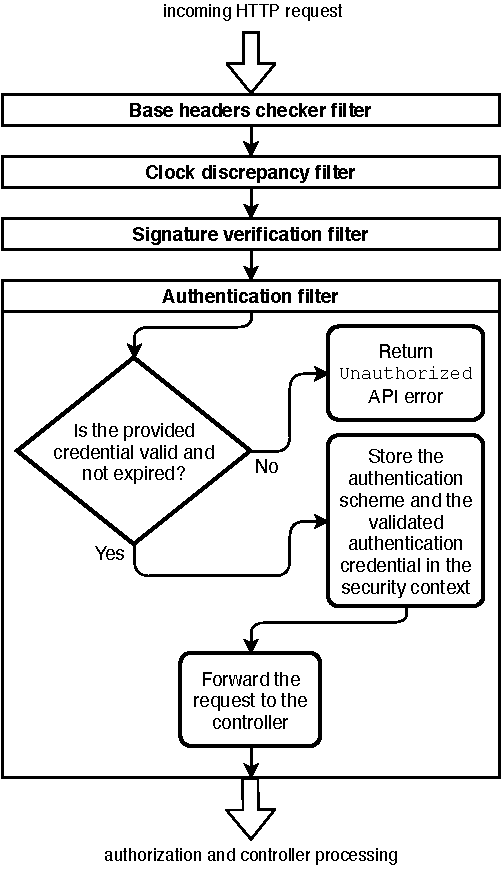
\includegraphics[height=\textheight-1cm]{figures/authentication-filter.pdf}
\end{figure}
